\documentclass[a3,convert]{standalone}
\usepackage{tikz}
\usetikzlibrary{calc,intersections,through}

\begin{document}
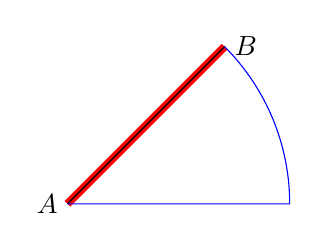
\begin{tikzpicture}

    \coordinate [label=left:$A$] (A) at (0,0);
    \coordinate [label=right:$B$] (B) at (2,2);

    \draw[red,line width=1mm] let \p1=($(B)-(A)$) in (A) --++ (45:({veclen(\x1,\y1)}););
    \draw (A) -- (B);
    \draw[blue] (A) let \p1 = ($(B)-(A)$) in --++({veclen(\x1,\y1)},0) arc (0:45:({veclen(\x1,\y1)}););

\end{tikzpicture}
\end{document}